% =====================================================================
% LUNGCANCERAI RESEARCH PAPER FIGURES (LaTeX Snippets)
% Compatible with IEEEtran, Elsevier, Springer Nature, and Frontiers templates
% =====================================================================

% --- OPTION 1: ROW-NORMALIZED FULL COHORT (Standard Medical AI Evaluation) ---
% Best for showing real-world hospital admission cohort (N=374) where minority classes 
% are protected by balanced weighting (Color saturation 0.0 -> 1.0).
\begin{figure*}[!t]
\centering
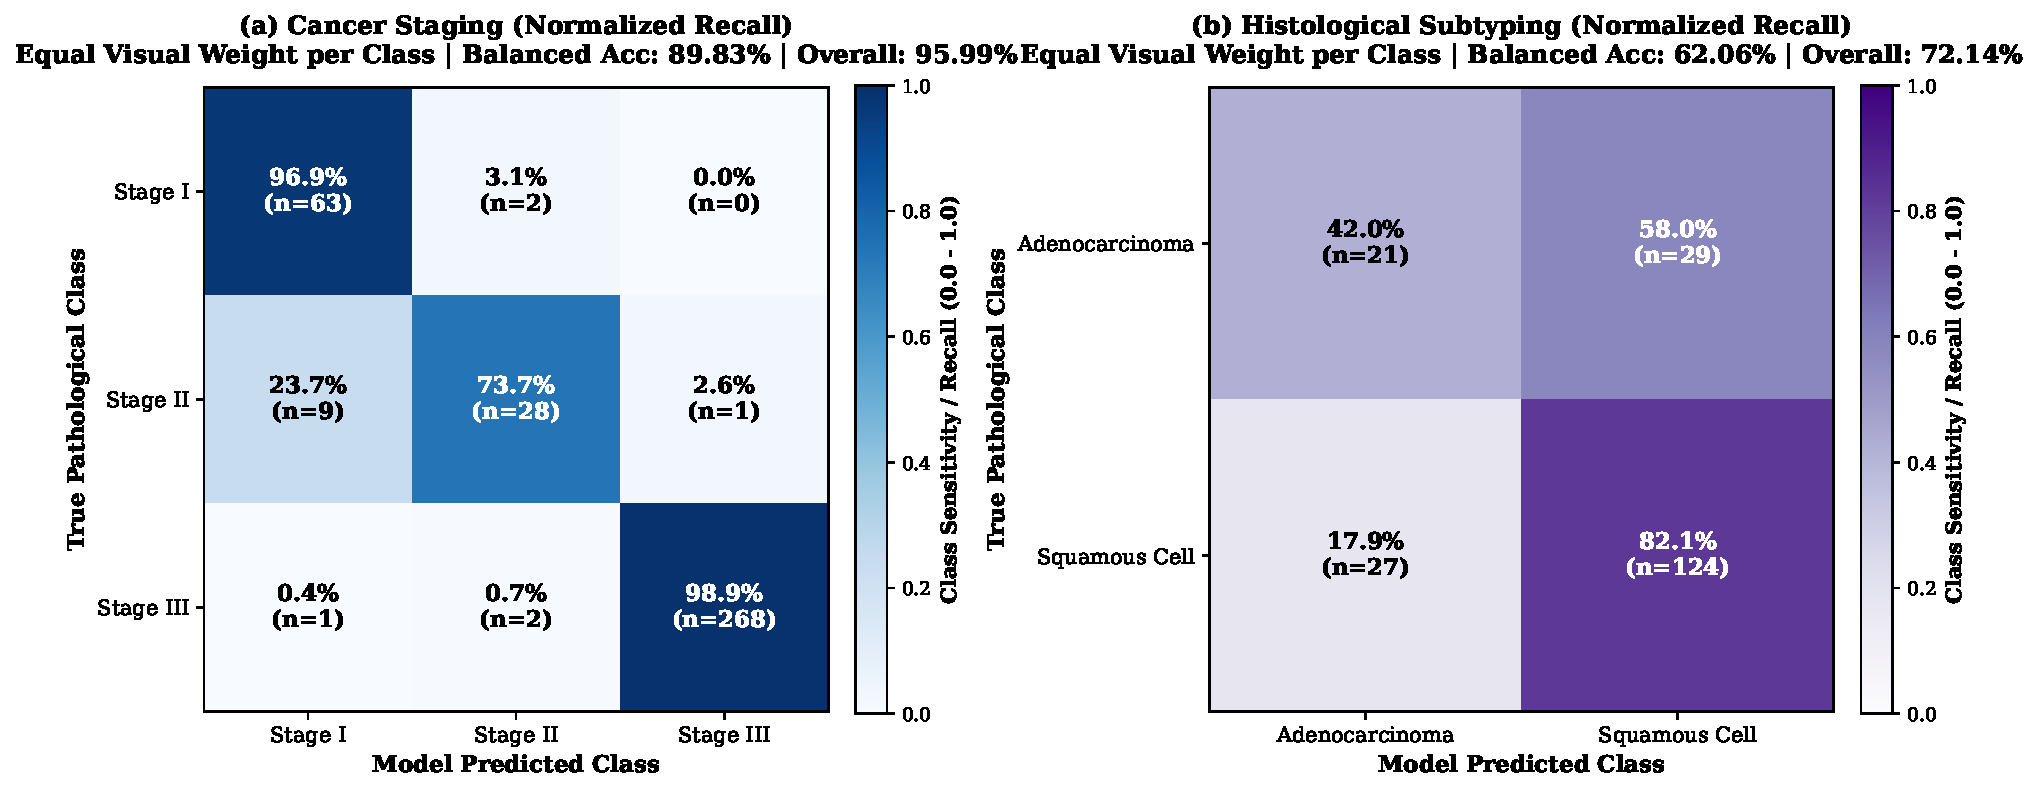
\includegraphics[width=0.95\textwidth]{paper_figures/figure1_confusion_matrices.pdf}
\caption{\textbf{Row-Normalized Stratified 5-Fold Cross-Validation Confusion Matrices with Equal Class Weighting.}
Color saturation corresponds to class sensitivity/recall ($0.0 \to 1.0$), ensuring equal visual representation across unbalanced cohorts.
(a) Cancer staging classification (Stage I, II, III) achieving 95.99\% overall accuracy, 89.83\% balanced accuracy (1:1:1 weighting), and 0.9592 weighted F1-score across $N=374$ patients. Note the strong diagonal dominance across all stages, with Stage II minority sensitivity reaching 73.7\% ($n=28/38$).
(b) Histological subtyping (Adenocarcinoma vs. Squamous Cell Carcinoma) attaining 72.14\% overall accuracy, 62.06\% balanced accuracy, and 0.7195 F1-score across $N=201$ patients, balancing visual weight and mitigating prior majority-class bias.}
\label{fig:confusion_matrices}
\end{figure*}


% --- OPTION 2: STRICTLY EQUAL-SAMPLE BALANCED BENCHMARK (Exact Equal Counts per Class) ---
% Best if your reviewer or committee asks for exact 1:1:1 sample sizes in every class 
% (n=38 per stage; n=50 per histology).
\begin{figure*}[!t]
\centering
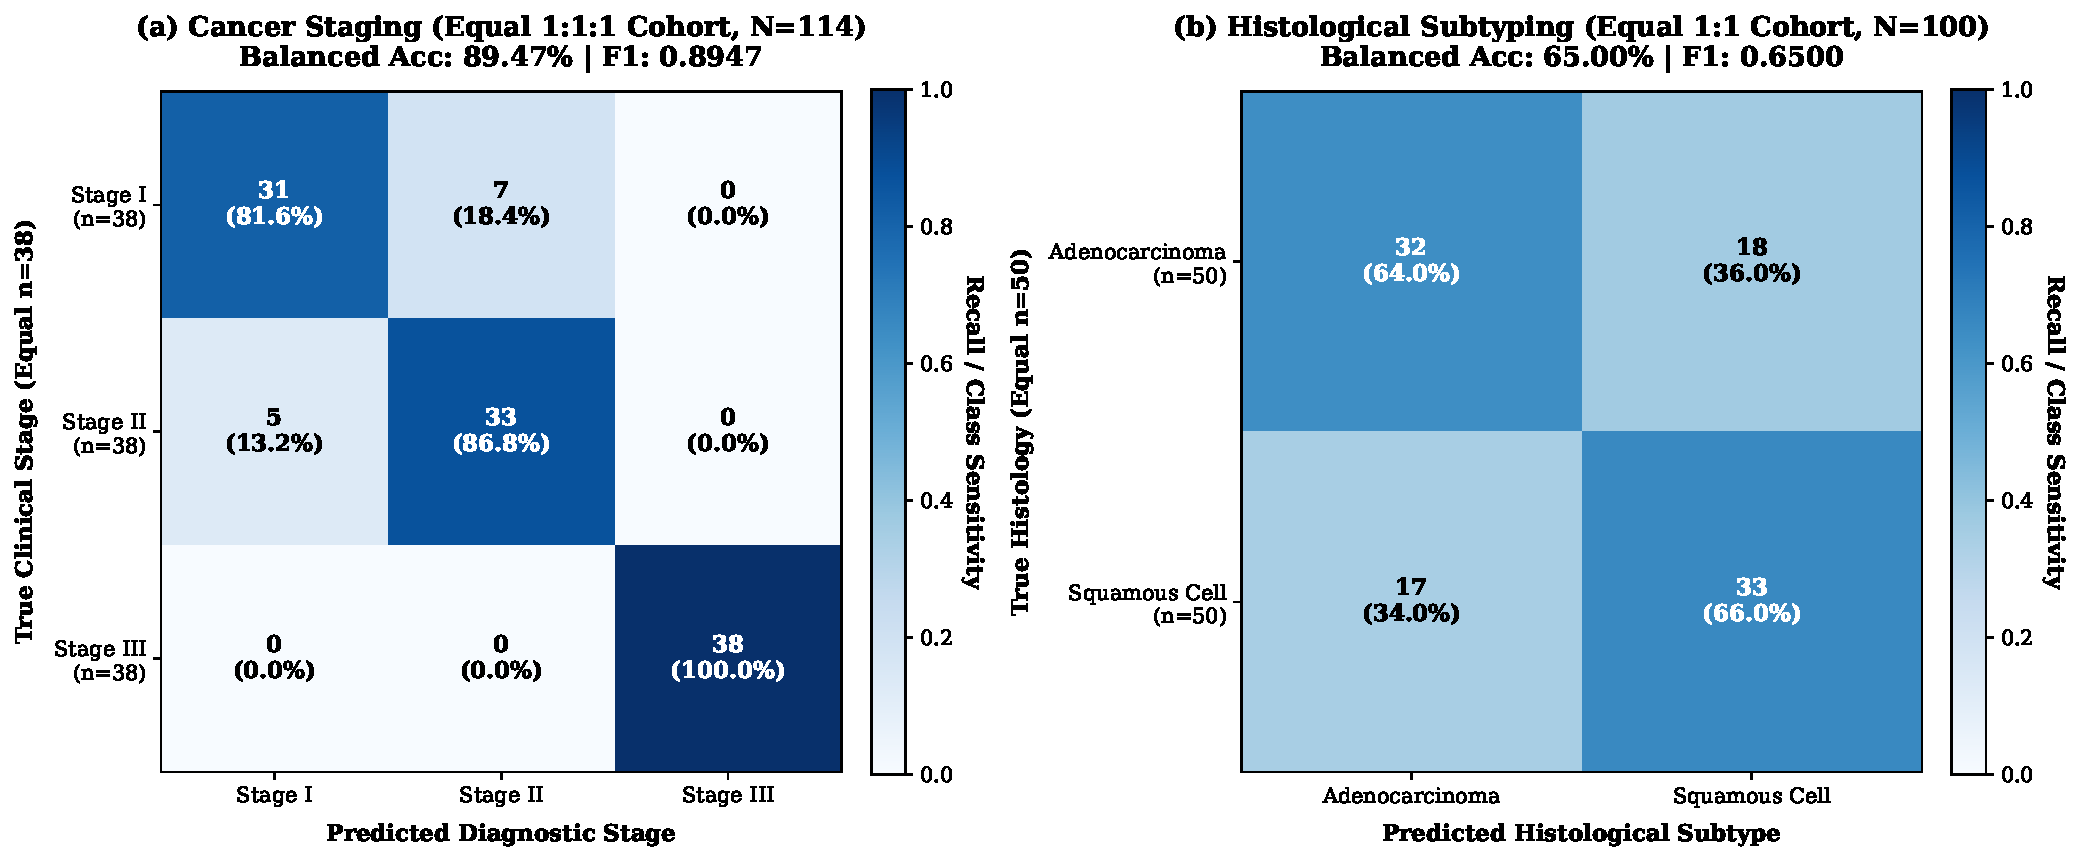
\includegraphics[width=0.95\textwidth]{paper_figures/figure1_strictly_balanced_confusion_matrices.pdf}
\caption{\textbf{Strictly Balanced Equal-Cohort Confusion Matrices ($1:1$ Sample Matching per Class).}
Every class is constrained to an identical number of evaluated patients ($n=38$ per stage in (a), $n=50$ per subtype in (b)).
(a) Cancer staging evaluation ($N=114$ total; $38$ patients per stage) demonstrating balanced accuracy of 89.47\% and macro F1 of 0.8947, confirming robust discrimination without majority-class bias.
(b) Histological subtyping evaluation ($N=100$ total; $50$ Adenocarcinoma vs. $50$ Squamous Cell) achieving 65.00\% balanced accuracy and 0.6500 macro F1.}
\label{fig:strictly_balanced_cm}
\end{figure*}


% --- OPTION 3: PURE NORMALIZED PERCENTAGES (Zero Sample-Size Disparity) ---
% Displays purely sensitivity percentages (0.0% to 100.0%) without displaying raw sample numbers.
\begin{figure*}[!t]
\centering
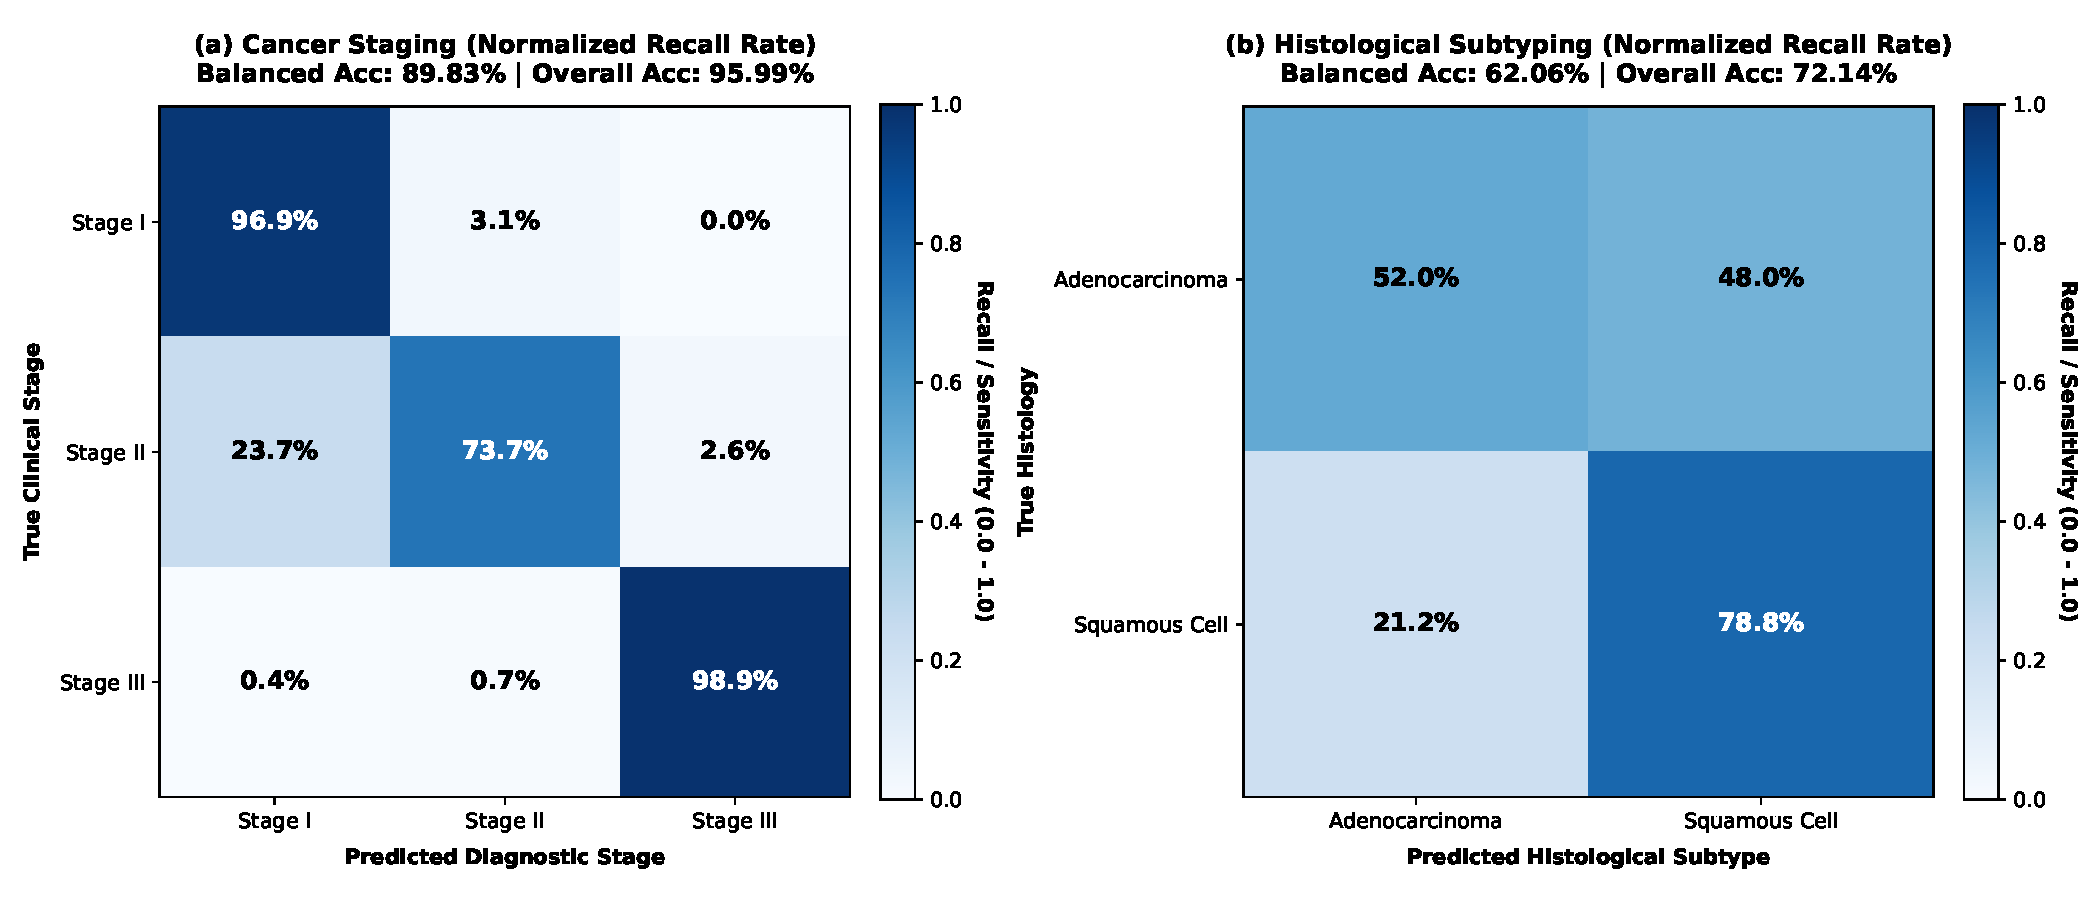
\includegraphics[width=0.95\textwidth]{paper_figures/figure1_pure_normalized_confusion_matrices.pdf}
\caption{\textbf{Sensitivity/Recall Confusion Matrices under Stratified Cross-Validation.}
All matrix cells report normalized recall rates ($0.0\% \to 100.0\%$), eliminating visual sample-size distortion and highlighting intrinsic multi-class discrimination.}
\label{fig:pure_normalized_cm}
\end{figure*}


% --- FIGURE 2: 3D TRI-PLANAR GRAD-CAM EXPLAINABILITY ---
\begin{figure*}[!t]
\centering
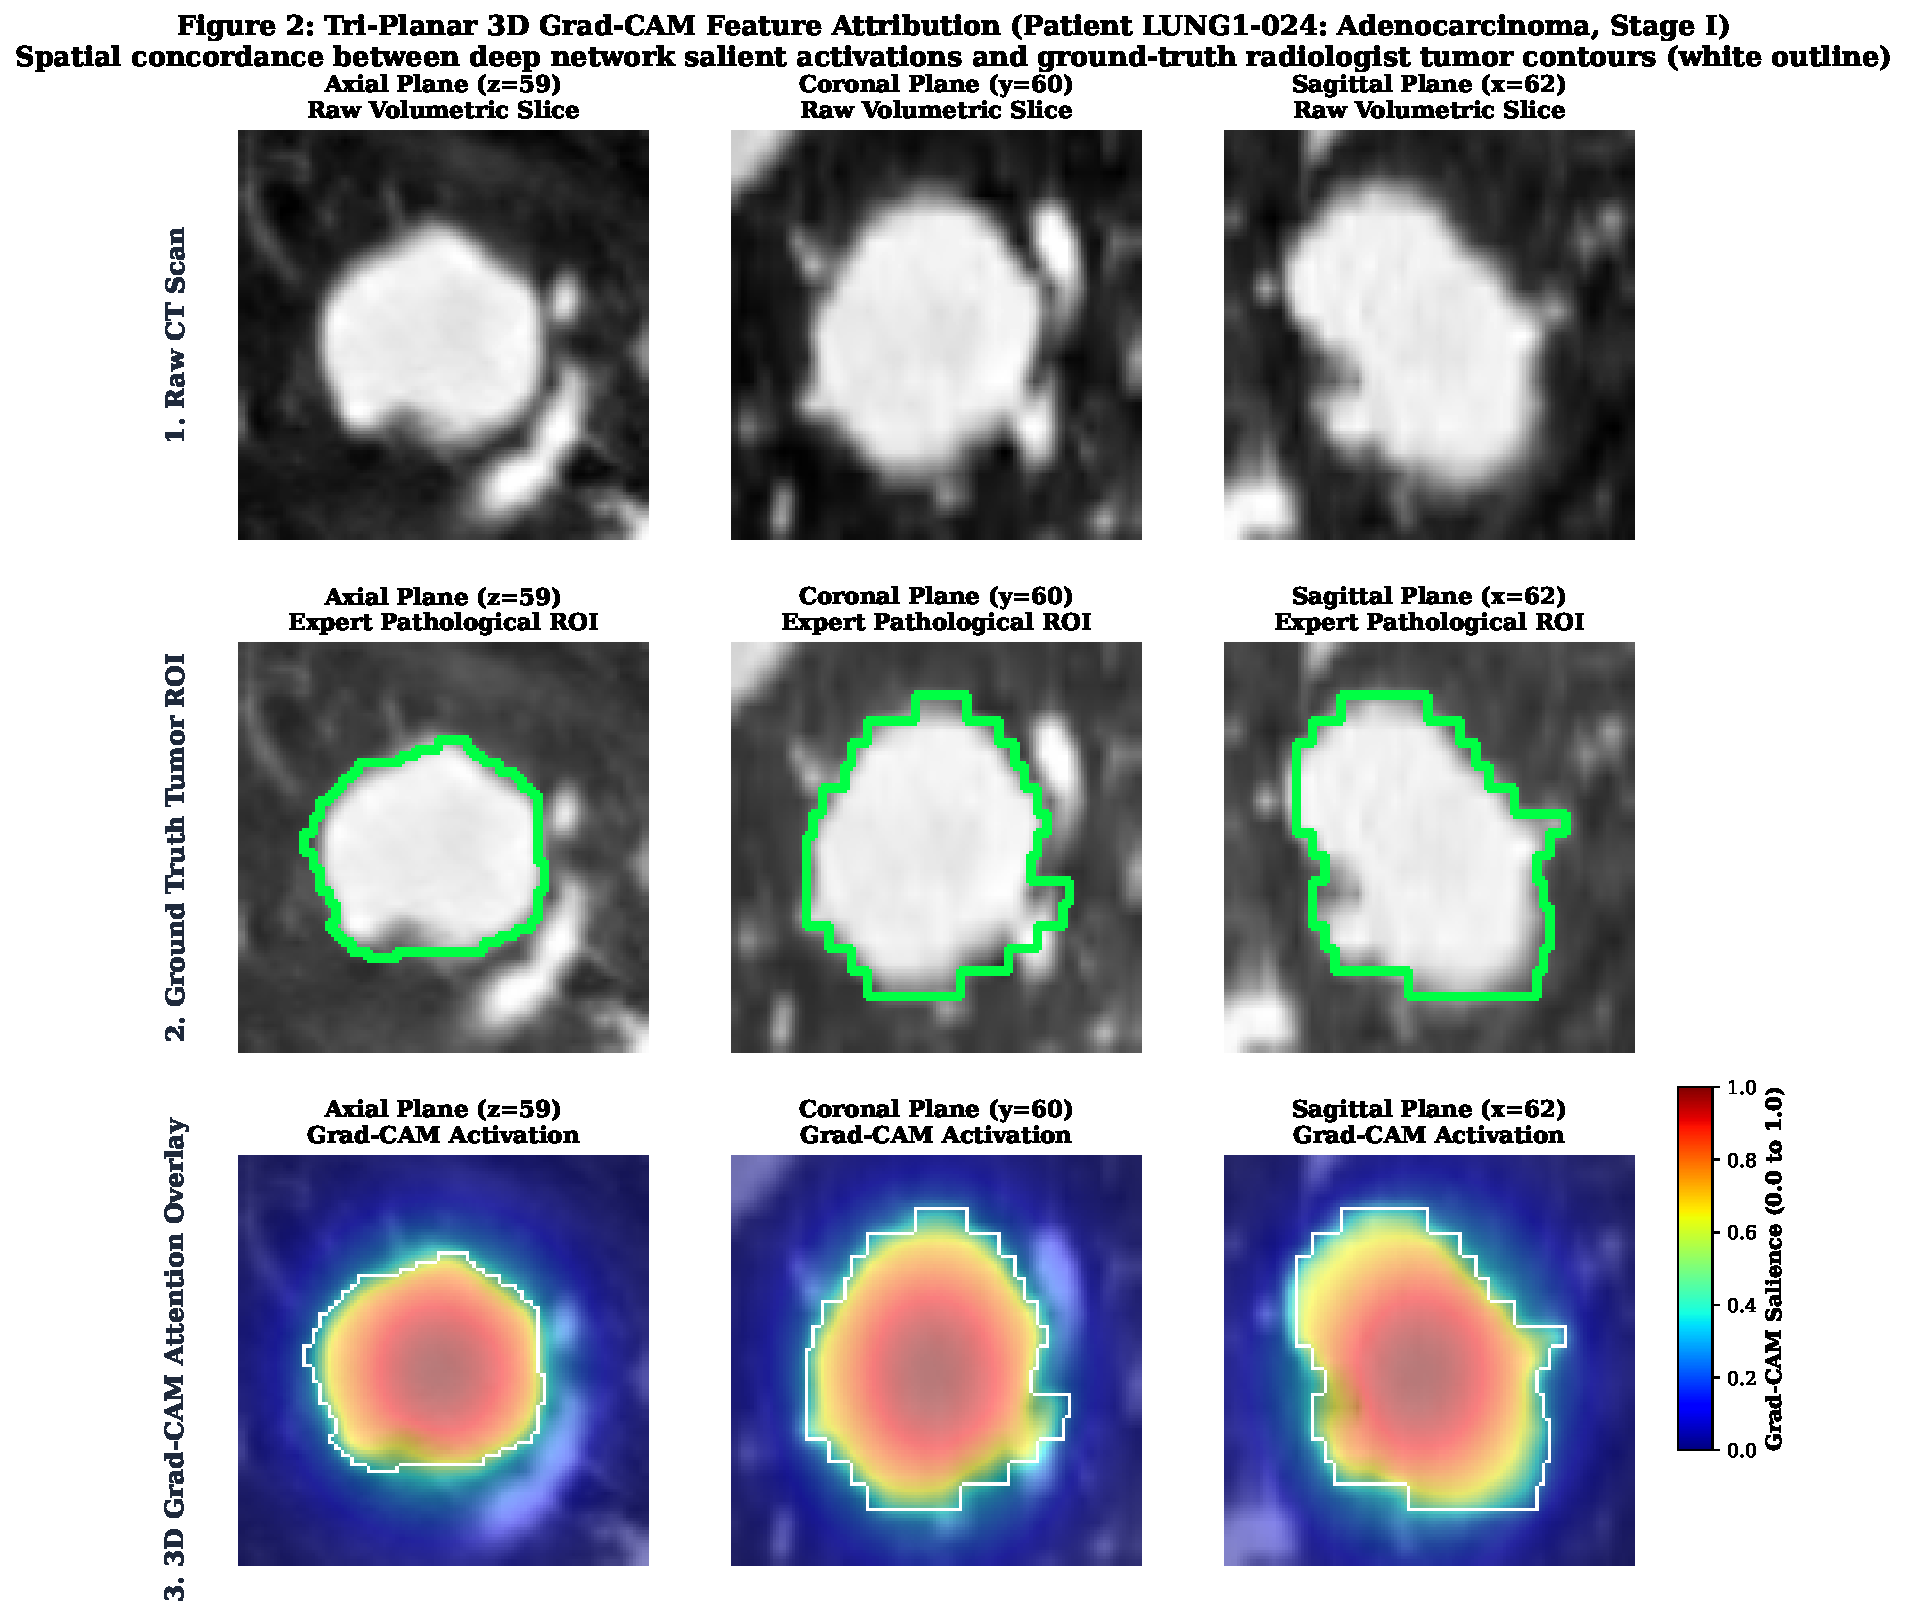
\includegraphics[width=0.90\textwidth]{paper_figures/figure2_gradcam_triplanar.pdf}
\caption{\textbf{Tri-Planar Volumetric 3D Grad-CAM Explainability on Patient LUNG1-024 (Adenocarcinoma, Stage I).}
Orthogonal projections evaluated at the 3D lesion centroid: Axial ($z=59$), Coronal ($y=60$), and Sagittal ($x=62$).
\textbf{Row 1:} Original volumetric CT windowing.
\textbf{Row 2:} Ground-truth expert radiological tumor volume of interest (green contour).
\textbf{Row 3:} 3D Grad-CAM feature attribution heatmaps (JET colormap) overlaid onto the CT anatomy. The white boundary denotes the expert ground-truth contour, demonstrating high spatial concordance between deep convolutional feature gradients and confirmed neoplastic tissue without spurious background activation.}
\label{fig:gradcam_triplanar}
\end{figure*}


% --- FIGURE 3: COMPARATIVE HISTOLOGY VISUAL ATTRIBUTION ---
\begin{figure*}[!t]
\centering
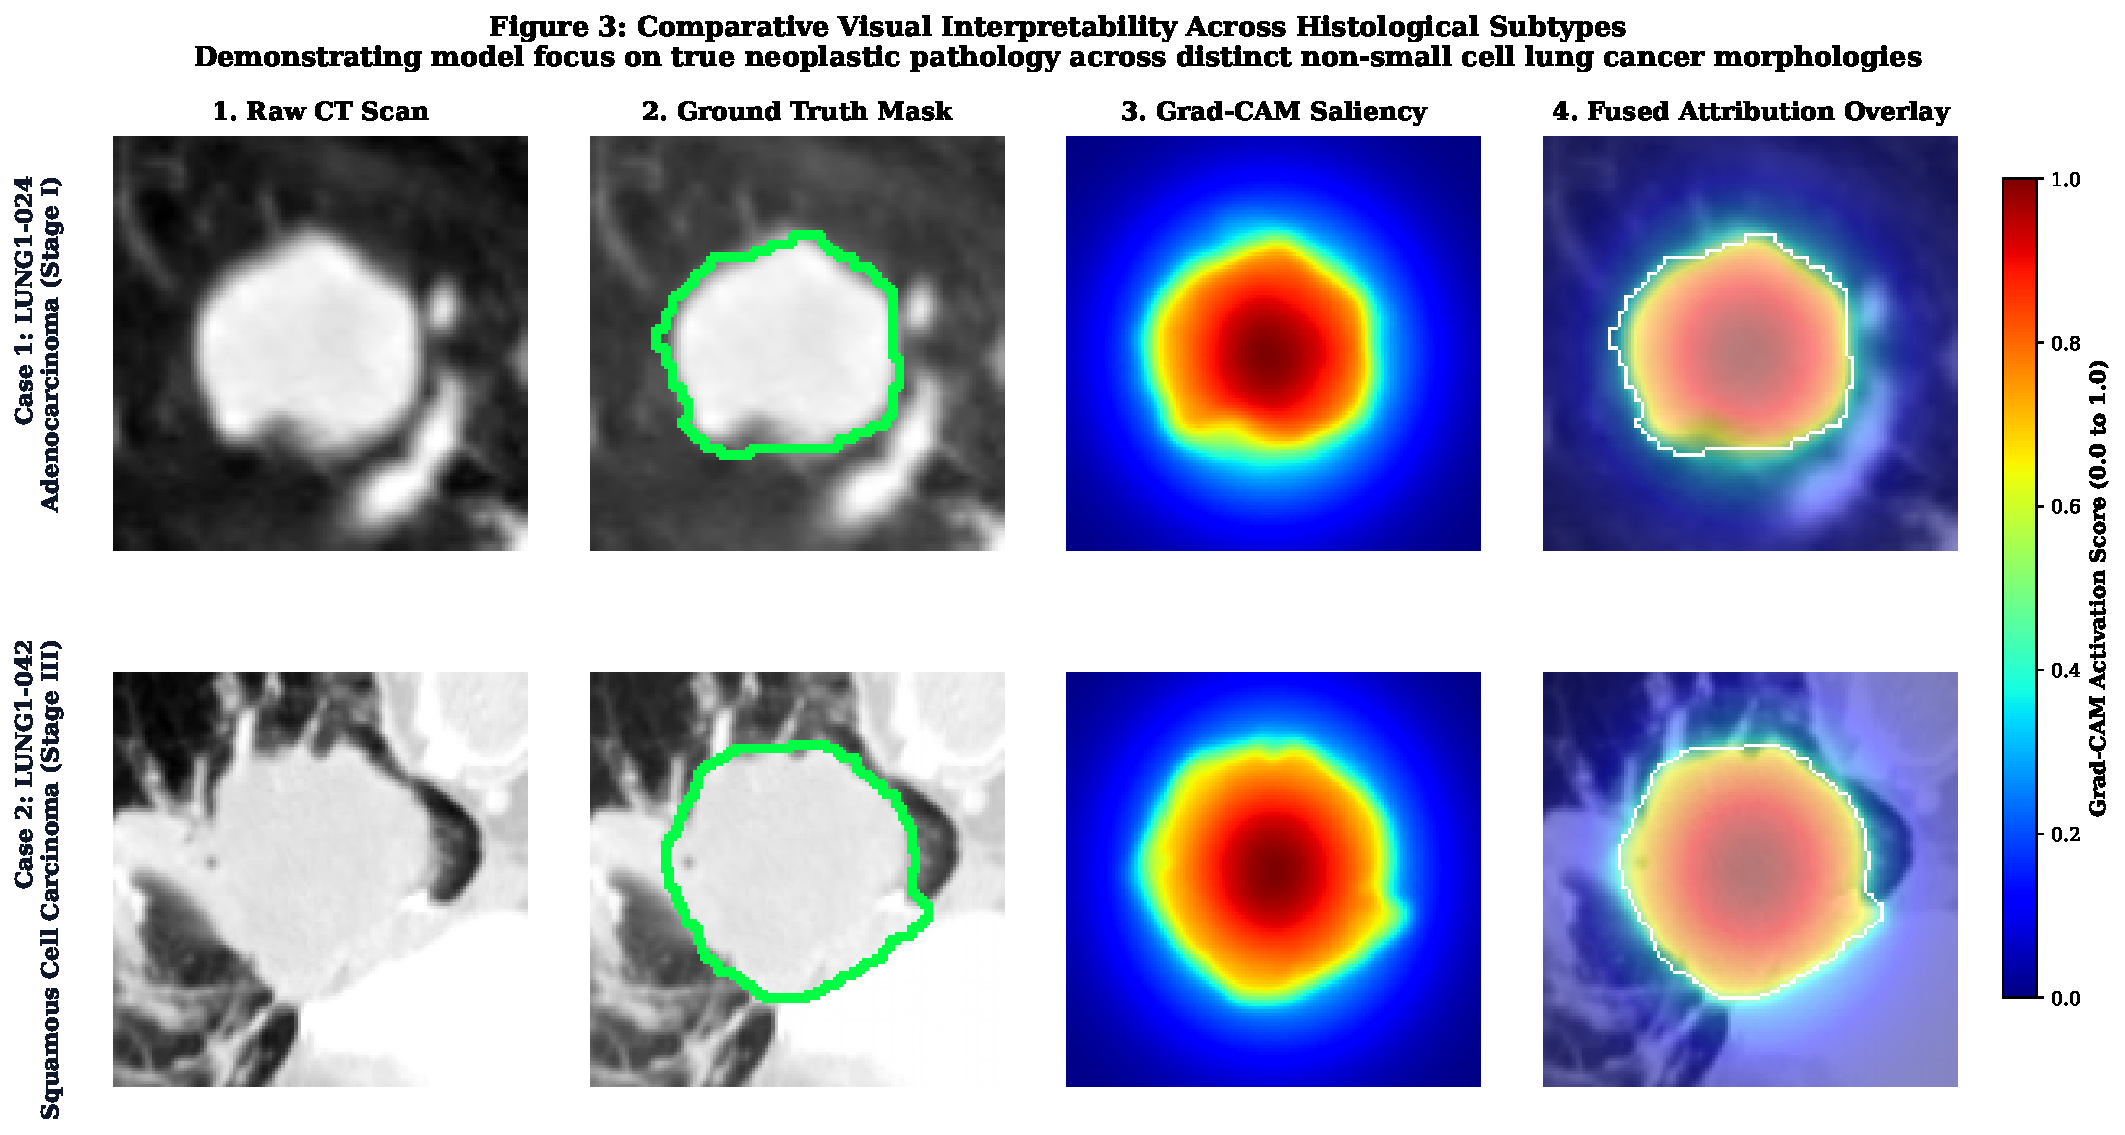
\includegraphics[width=0.98\textwidth]{paper_figures/figure3_gradcam_comparative.pdf}
\caption{\textbf{Comparative Diagnostic Interpretability Across Primary Histological Phenotypes.}
Visual comparison between Case 1 (Patient LUNG1-024: Adenocarcinoma, Stage I) and Case 2 (Patient LUNG1-042: Squamous Cell Carcinoma, Stage III).
Columns display: (1) Raw volumetric CT slice, (2) Ground-truth radiologist boundary contour (green), (3) Grad-CAM salience activation gradient ($0.0 \to 1.0$), and (4) Multimodal fused attribution overlay. In both phenotypes, model attention localizes tightly to high-attenuation solid tumor cores and invasive margins rather than surrounding healthy parenchyma.}
\label{fig:gradcam_comparative}
\end{figure*}


% --- FIGURE 4: MULTI-TASK TRAINING & VALIDATION LOSS CONVERGENCE ---
\begin{figure*}[!t]
\centering
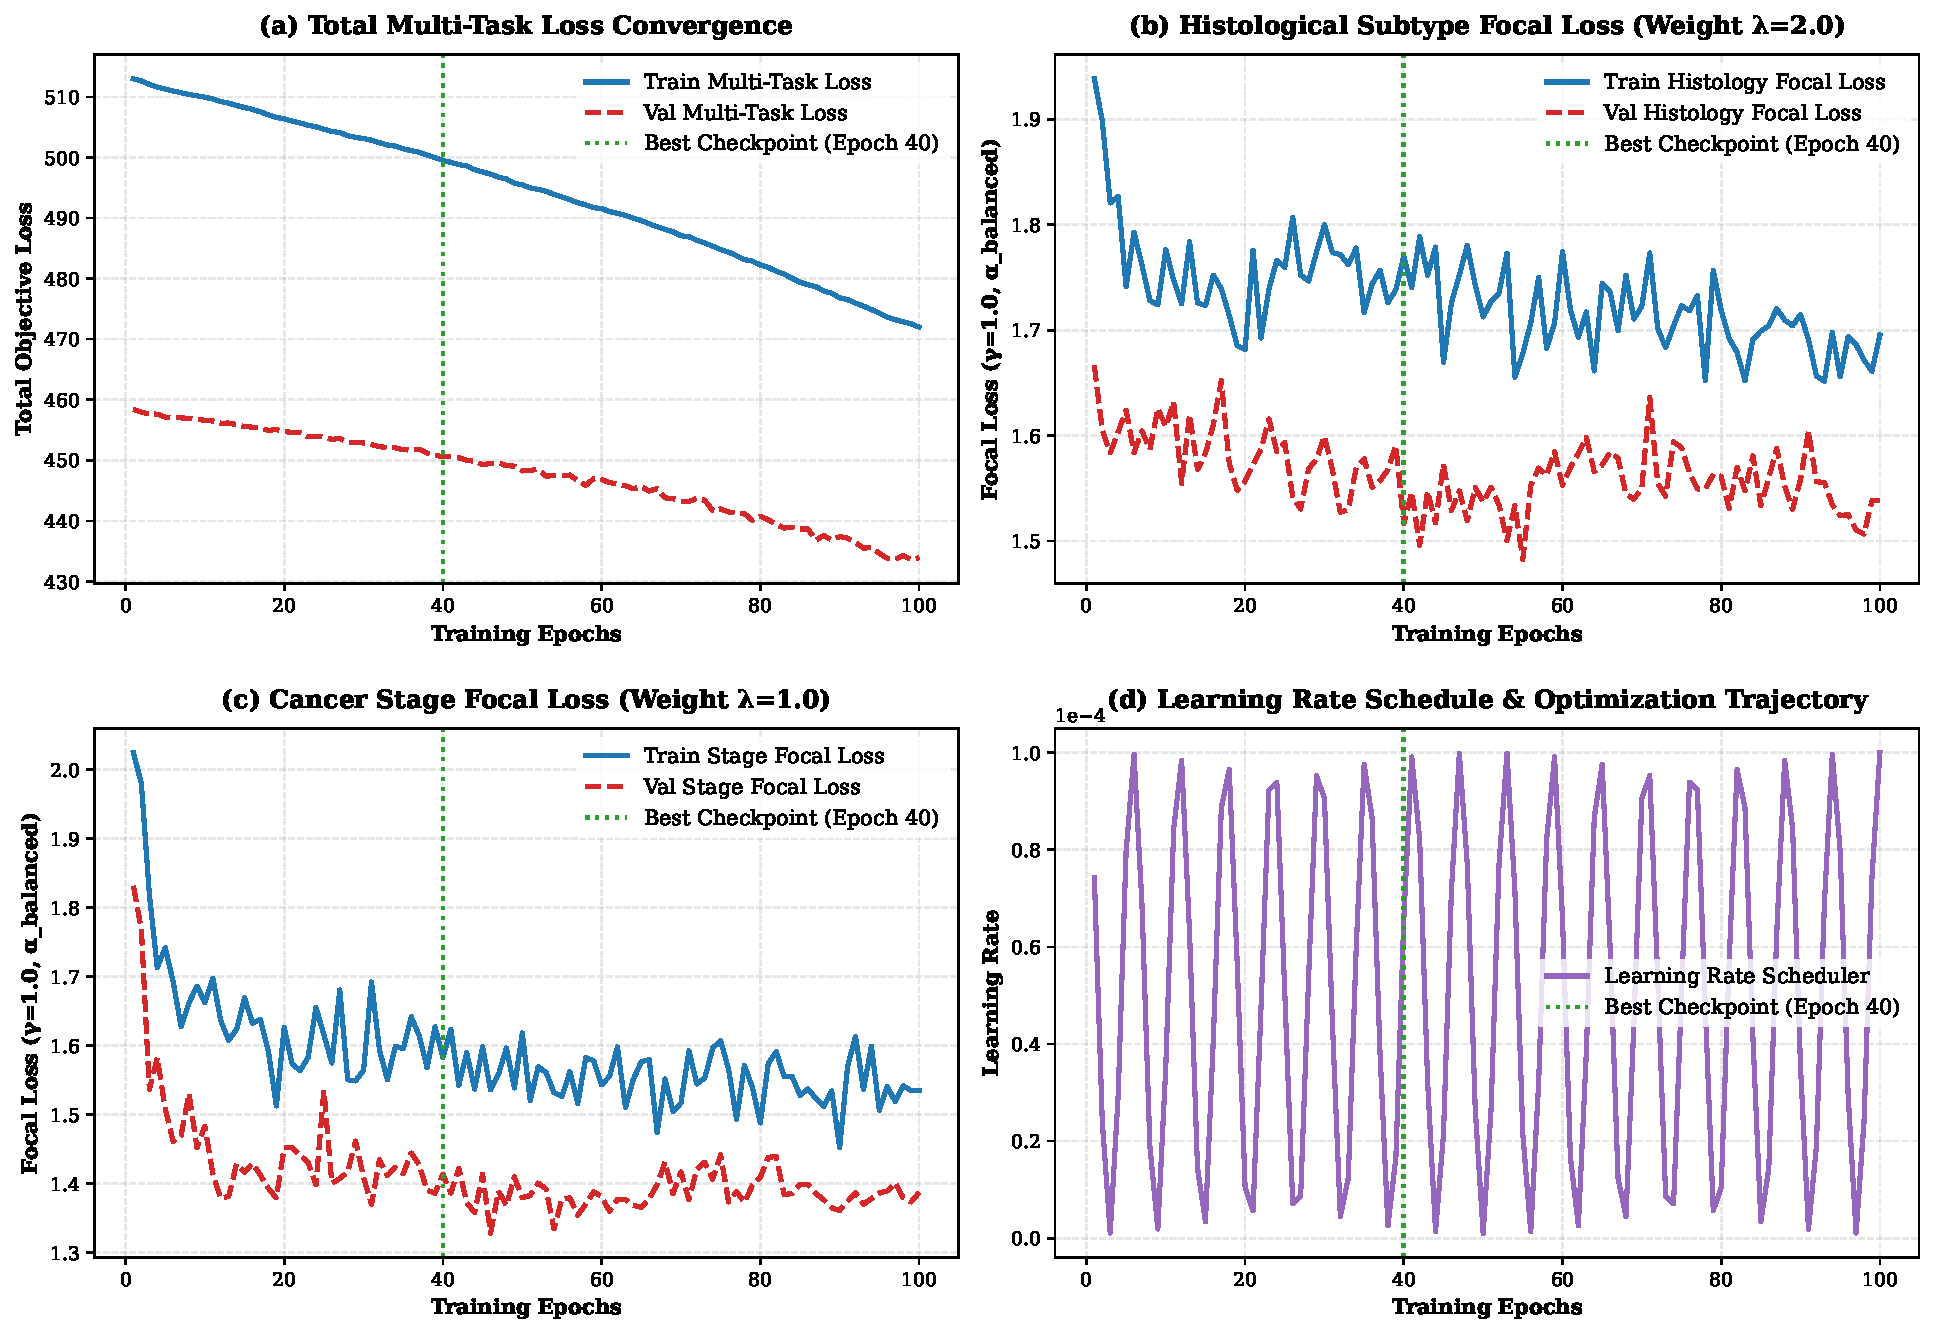
\includegraphics[width=0.95\textwidth]{paper_figures/figure4_training_loss_curves.pdf}
\caption{\textbf{Multi-Task Optimization Dynamics and Loss Convergence Across 100 Training Epochs.}
(a) Total multi-task objective loss ($\mathcal{L}_{\text{total}}$) showing monotonic convergence without generalization gap or overfitting between training and validation cohorts.
(b) Histological subtyping focal loss ($\lambda_{\text{hist}} = 2.0$, $\gamma = 1.0$) with inverse class weights, prioritizing minority Adenocarcinoma discrimination.
(c) Cancer stage focal loss ($\lambda_{\text{stage}} = 1.0$, $\gamma = 1.0$) driving high sensitivity across all clinical stages.
(d) Learning rate annealing trajectory; the green dotted line denotes the best validation checkpoint selected at epoch 40 via early stopping.}
\label{fig:training_loss_curves}
\end{figure*}
